\documentclass[11pt]{article}
\usepackage[T1]{fontenc}
\usepackage{lmodern}
\usepackage{amsmath,amssymb,amsthm}
\usepackage{graphicx}
\usepackage[margin=1in]{geometry}
\usepackage{microtype}
\usepackage[colorlinks=true,urlcolor=blue,citecolor=blue]{hyperref}

\newtheorem{theorem}{Theorem}
\newtheorem{lemma}{Lemma}
\newcommand{\F}{\mathbb F}
\newcommand{\N}{\mathbb N}
\newcommand{\Ran}{\operatorname{Ran}}

\title{A disconnected nonzero fixed-diagonal idempotent fiber\\
in infinite-dimensional Hilbert space}
\author{Candidate counterexample for arXiv:0906.0139}
\date{17 August 2026}

\begin{document}
\maketitle

\begin{center}
\fbox{\parbox{0.91\linewidth}{\textbf{Status: candidate counterexample,
likely valid; human review pending.}  The construction is self-contained and
works over both real and complex scalars.}}
\end{center}

\section*{Source question}

Giol, Kovalev, Larson, Nguyen, and Tener prove that for every diagonal
$d\in D_n(\mathbb C)$, the finite-dimensional fiber
\[
 \{q\in M_n(\mathbb C):q^2=q,\ E(q)=d\}
\]
is path-connected.  At the end of their introduction they ask whether full
analogues of this theorem and their half-diagonal projection theorem hold on
separable infinite-dimensional Hilbert spaces, in the operator-norm topology
\cite{GKLNT}.  The relevant source context spans PDF pages 2--3:

\begin{center}
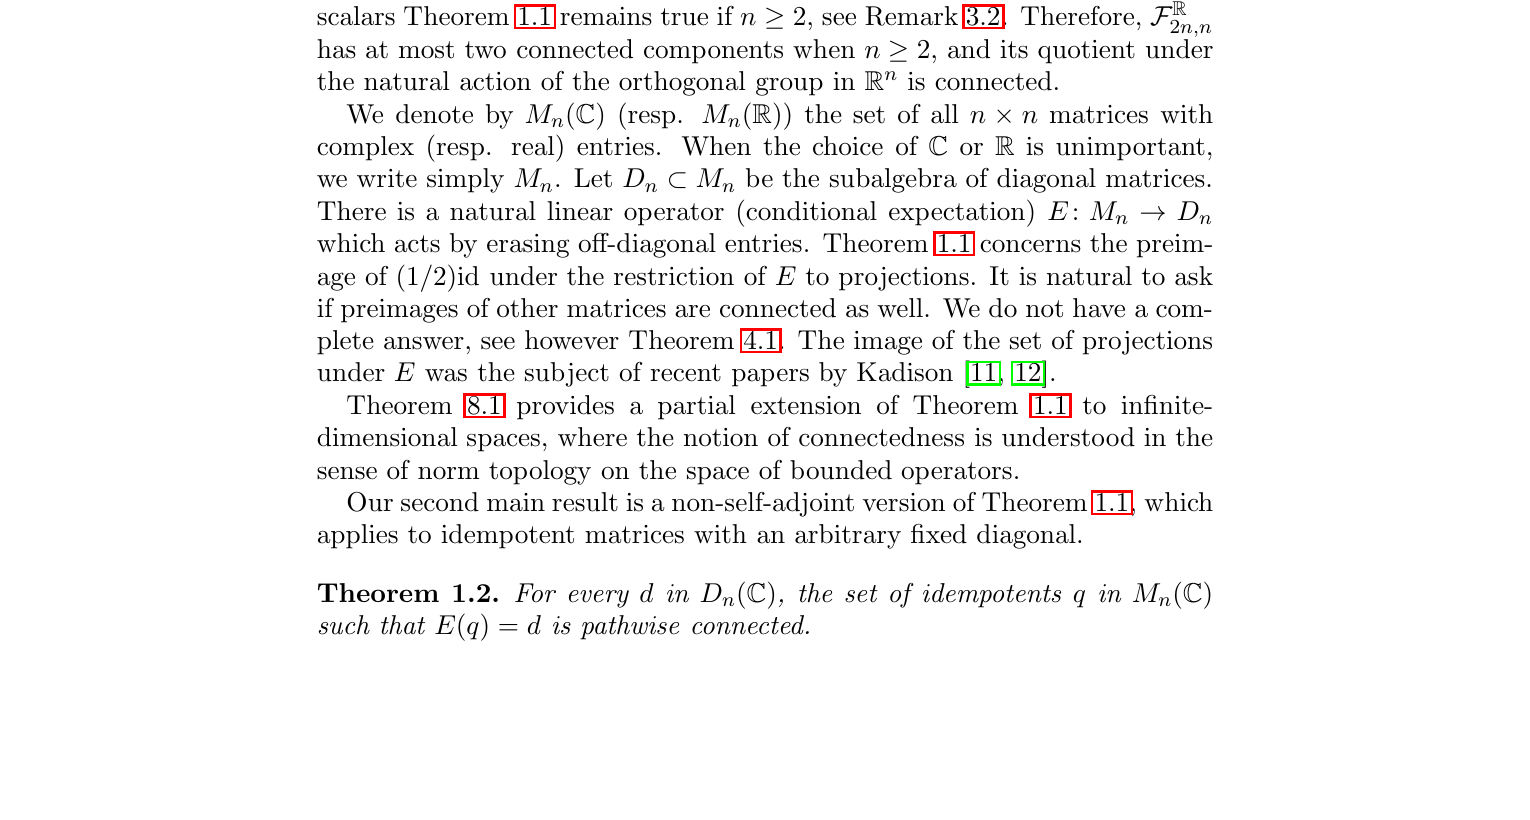
\includegraphics[width=0.98\linewidth]{figures/open_problem_crop_part1.png}

\smallskip
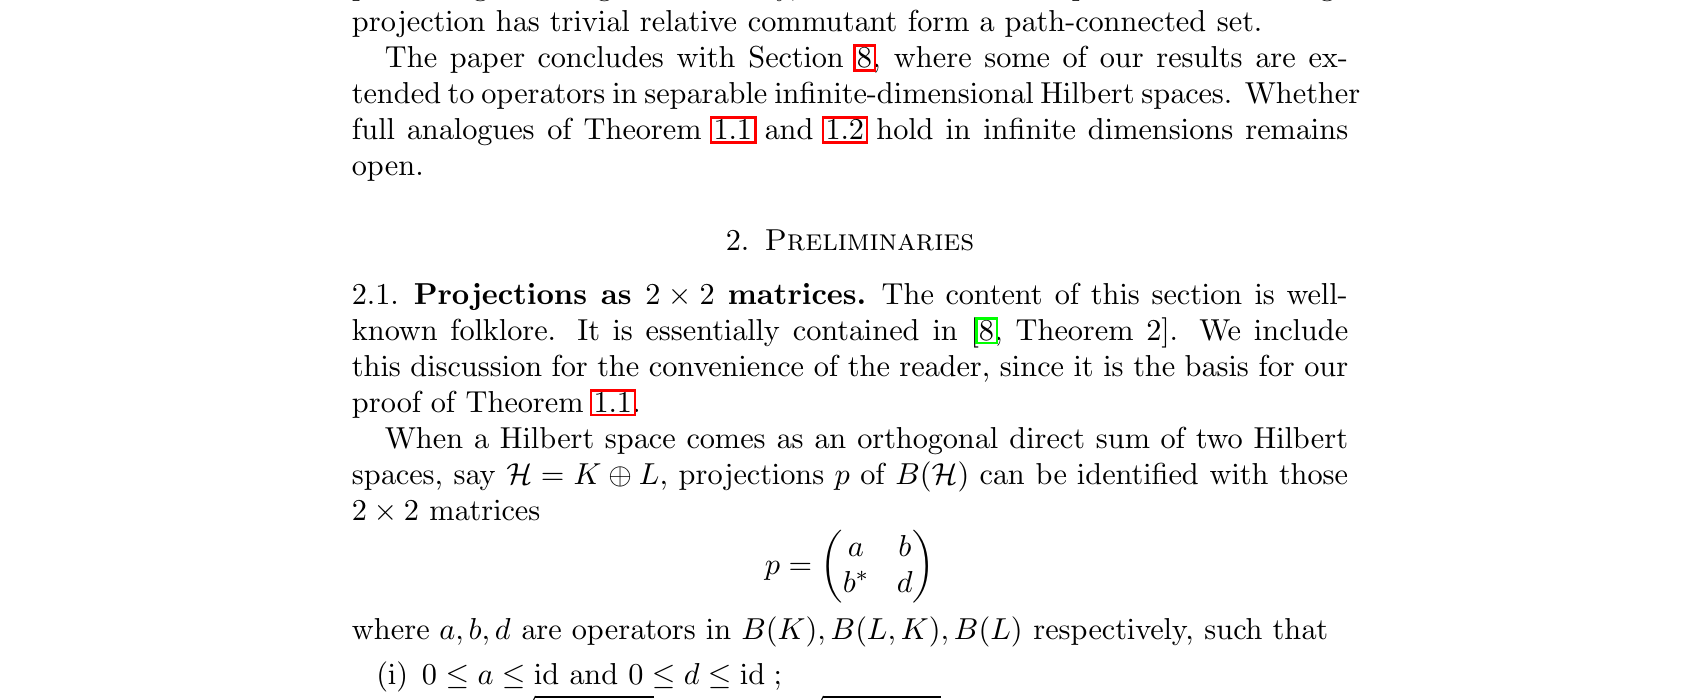
\includegraphics[width=0.98\linewidth]{figures/open_problem_crop_part2.png}
\end{center}

The idempotent half of that literal question has a negative answer, even for
a fixed diagonal which is not identically zero.

\section*{Idea of the proof}

The key is to exploit a phenomenon unavailable in finite dimensions: an
infinite-rank idempotent can have zero diagonal.  We build one explicitly from
infinitely many copies of a rank-one $2\times2$ oblique projection.  A
countable regrouping places two coordinates carrying diagonal weight $-1$
beside one carrying weight $2$; an orthogonal $3\times3$ mixing gives every
new basis vector weights $2/3$ and $1/3$, so its diagonal value is
$-(2/3)+2(1/3)=0$.

After adjoining a one-dimensional identity summand, this idempotent and the
rank-one coordinate projection have the same nonzero diagonal
$(1,0,0,\ldots)$.  They cannot be joined by a norm-continuous path of
idempotents because rank is locally constant in the idempotent set.

\section*{Counterexample}

Throughout, $\F$ is either $\mathbb R$ or $\mathbb C$, and diagonals are
taken relative to the displayed orthonormal basis.

\begin{theorem}
There exist a separable infinite-dimensional Hilbert space $H$ over $\F$, an
orthonormal basis $(e_j)_{j\ge0}$, and the nonzero diagonal
$d=(1,0,0,\ldots)$ such that
\[
 \mathcal I_d=\{T\in B(H):T^2=T,\ 
       \langle Te_j,e_j\rangle=d_j\ \text{for all }j\}
\]
is not path-connected in the operator norm.  More precisely, $\mathcal I_d$
contains a rank-one idempotent and an infinite-rank idempotent, which lie in
different norm-path components.
\end{theorem}

\begin{proof}
Let $K=\ell_2(\N)\oplus\ell_2(\N)$, with its usual orthonormal vectors
$u_i,v_i$ for $i\in\N=\{0,1,2,\ldots\}$.  Define $R\in B(K)$ blockwise by
\begin{equation}\label{eq:R}
 Ru_i=-u_i-2v_i,\qquad Rv_i=u_i+2v_i.
\end{equation}
On $\operatorname{span}\{u_i,v_i\}$ this is the matrix
\[
 A=\begin{pmatrix}-1&1\\-2&2\end{pmatrix},
 \qquad A^2=A.
\]
Thus $R^2=R$.  Every block has one-dimensional range
$\F(u_i+2v_i)$, so $R$ has infinite rank.

We now exhibit an orthonormal basis in which $R$ has zero diagonal.  Define a
bijection $\phi:\N\times\{0,1\}\to\N$ by
\[
\begin{array}{c|cccc}
(m,j)&(0,0)&(0,1)&(1,0)&(1,1)\\ \hline
\phi(m,j)&1&2&3&0,
\end{array}
\]
and, for $m\ge2$, by
\[
 \phi(m,0)=2m+1,\qquad \phi(m,1)=2m.
\]
For every $m$ and $j$ one has $\phi(m,j)\ne m$.  The three-dimensional
spaces
\[
 G_m=\operatorname{span}\{u_{\phi(m,0)},u_{\phi(m,1)},v_m\}
\]
are mutually orthogonal and their orthogonal direct sum is $K$.

In each $G_m$, let $w_{m,0},w_{m,1},w_{m,2}$ be the vectors whose coordinate
columns relative to the displayed ordered spanning set are the columns of
\begin{equation}\label{eq:O}
 O=\begin{pmatrix}
 1/\sqrt2&-1/\sqrt2&0\\
 1/\sqrt6& 1/\sqrt6&-2/\sqrt6\\
 1/\sqrt3& 1/\sqrt3& 1/\sqrt3
 \end{pmatrix}.
\end{equation}
The matrix $O$ is real orthogonal.  Hence all the $w_{m,r}$ form an
orthonormal basis of $K$, over either scalar field.  Each column of $O$ has
total squared weight $2/3$ in its first two coordinates and squared weight
$1/3$ in its last coordinate.

Write one such vector as
\[
 w=\alpha u_{\phi(m,0)}+\beta u_{\phi(m,1)}+\gamma v_m.
\]
The two inequalities $\phi(m,j)\ne m$ ensure that none of the cross terms in
\eqref{eq:R} contributes to $\langle Rw,w\rangle$.  Consequently
\[
 \langle Rw,w\rangle
 =-|\alpha|^2-|\beta|^2+2|\gamma|^2
 =-\frac23+2\frac13=0.
\]
Thus $R$ is an infinite-rank idempotent with zero diagonal in the basis
$(w_{m,r})$.

Finally let $H=\F z\oplus K$, where $z$ is a unit vector, and order the basis
as
\[
 e_0=z,\qquad e_{3m+r+1}=w_{m,r}\quad(m\ge0,\ 0\le r\le2).
\]
Consider
\[
 P=I_{\F z}\oplus0_K,\qquad Q=I_{\F z}\oplus R.
\]
Both are idempotents and both have diagonal $(1,0,0,\ldots)$.  But
$\dim\Ran P=1$, whereas $\dim\Ran Q=\aleph_0$.

It remains to show that this prevents a norm-continuous idempotent path.  If
$S,T$ are idempotents with $\|S-T\|<1$, then
$T:\Ran S\to\Ran T$ is injective: for $x\in\Ran S$ with $Tx=0$,
\[
 \|x\|=\|Sx\|=\|(S-T)x\|<\|x\|,
\]
unless $x=0$.  Interchanging $S$ and $T$ gives injections in both directions,
so their Hilbert-space ranks agree.  Any norm-continuous path on $[0,1]$ is
uniformly continuous and can be subdivided into finitely many consecutive
steps of norm less than one.  Rank is therefore constant along every such
idempotent path.  Since $P$ and $Q$ have different ranks, they lie in
different path components of $\mathcal I_d$.
\end{proof}

\section*{Verification}

The proof uses only the block identity $A^2=A$, orthogonality of $O$, the
explicit bijection $\phi$, and the local rank lemma.  The included script
\texttt{code/verify\_construction.py} checks the block identity and rank,
the orthogonality and weight cancellation in \eqref{eq:O}, bijectivity and
absence of forbidden pairings through 2,000 groups, and 6,000 initial
diagonal values.  Run it from the repository root with
\begin{verbatim}
conda run --no-capture-output -n sandbox python \
  runs/fa_banach_001/solutions/counterexamples/
  0906.0139_infinite_fixed_diagonal_idempotents_disconnected/
  code/verify_construction.py
\end{verbatim}
where the three path lines are concatenated.  These checks are corroborative;
the displayed identities constitute the proof.

\section*{Scope and novelty check}

This counterexample settles only the idempotent half of the source's final
infinite-dimensional question.  It does not decide whether all projections
with constant diagonal $1/2$ are norm-path-connected.  Eight focused upgrade
attempts tested block-index, compact-perturbation, paving, and finite
approximation routes; no global invariant or uniform homotopy was obtained for
that projection fiber.

The finite frame-homotopy problem is no longer open: Cahill, Mixon, and Strawn
explicitly cite the source and completely resolve it \cite{CMS}.  Needham and
Shonkwiler's prescribed-frame theorem also implies, after the usual Gramian
quotient, that every nonempty finite-dimensional complex projection fiber with
arbitrary prescribed diagonal is path-connected \cite{NS}.

The bounded search was run on 17 August 2026.  It covered the run indexes and
primary-source/arXiv queries using the source identifier and exact variants of
``fixed diagonal idempotents path connected,'' ``zero-diagonal idempotents,''
and the source's question.  It found the known zero-diagonal existence
theory---the source itself notes such examples, and Loreaux--Weiss later prove
much stronger diagonal-realization results \cite{LW}---but no explicit
statement of the nonzero-fiber rank-component counterexample above.  Novelty
confidence is therefore limited: the construction and topological conclusion
here are self-contained, but the underlying zero-diagonal phenomenon is known.

\section*{Human-review recommendation}

Check (i) that $\phi$ is a bijection and the $G_m$ exhaust $K$,
(ii) that the forbidden equalities $\phi(m,j)=m$ are exactly what eliminates
the cross terms, and (iii) that the intended infinite analogue of Theorem 1.2
does not silently restrict to one fixed rank/nullity stratum.  Under the
literal formulation recorded in the source introduction, the counterexample
is complete.

\begin{thebibliography}{9}
\bibitem{GKLNT}
J. Giol, L. V. Kovalev, D. Larson, N. Nguyen, and J. E. Tener,
\emph{Projections and idempotents with fixed diagonal and the homotopy
problem for unit tight frames}, Operators and Matrices 5 (2011), 139--155;
arXiv:0906.0139.

\bibitem{CMS}
J. Cahill, D. G. Mixon, and N. Strawn,
\emph{Connectivity and irreducibility of algebraic varieties of finite unit
norm tight frames}, SIAM J. Appl. Algebra Geom. 1 (2017), 38--72;
arXiv:1311.4748.

\bibitem{NS}
T. Needham and C. Shonkwiler,
\emph{Symplectic geometry and connectivity of spaces of frames},
Adv. Comput. Math. 47 (2021), article 5; arXiv:1804.05899.

\bibitem{LW}
J. Loreaux and G. Weiss,
\emph{Diagonality and idempotents with applications to problems in operator
theory and frame theory}, J. Operator Theory 75 (2016), 91--118;
arXiv:1410.7441.
\end{thebibliography}

\end{document}
